\documentclass[a4,paper]{article}

\usepackage{layout}

\DeclareSIUnit\year{Jahr}

\title{Notizen EEV -- SW01}
\date{\today}
\author{Daniel Winz}

\begin{document}
\maketitle
\clearpage

\section{Allgemeine Informationen}
\subsection{ABB - Schaltanlagen}
\href{www.abb.de/schaltanlagen}{www.abb.de/schaltanlagen}

\subsection{Exkursionen}
\begin{itemize}
    \item Rathausen
    \item Mettlen \\
        4.12.2015
\end{itemize}

\section{Swissix}
Day ahead

\section{Ziele der Stromversorgung}
\begin{itemize}
    \item ausreichende Menge
    \item dauernd verfügbar \\
        CH: ca. $1.7\frac{\si{\hour}}{\si{\year}}$ nicht verfügbar
    \item konstante Kennwerte
    \item gestörte Netzteile müssen selektiv getrennt werden: Schutz
    \item Vermeidung von Gefahren
    \item Bestmöglicher Wirkungsgrad
    \item Geringe Umweltbelastung
\end{itemize}
\clearpage

\section{Drehstromsystem}
\begin{figure}[h!]
    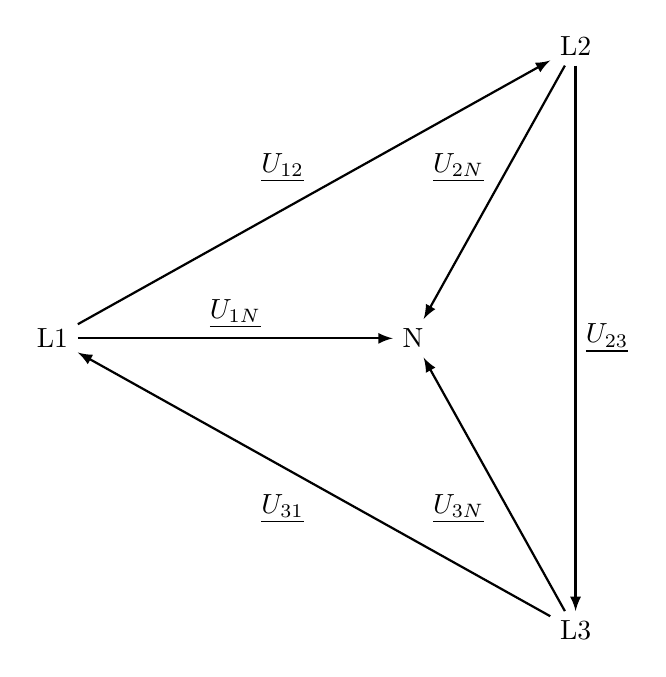
\begin{tikzpicture}
        \node(l1) at (180:4) [left]        {L1};
        \node(l2) at ( 60:4) [above right] {L2};
        \node(l3) at (300:4) [below right] {L3};
        \node(n)  at (  0:0) [right]       {N};
        \draw[thick, -latex] (l1) -- node[above left] {$\underline{U_{12}}$} (l2);
        \draw[thick, -latex] (l2) -- node[right]      {$\underline{U_{23}}$} (l3);
        \draw[thick, -latex] (l3) -- node[below left] {$\underline{U_{31}}$} (l1);
        \draw[thick, -latex] (l1) -- node[above]      {$\underline{U_{1N}}$} (n);
        \draw[thick, -latex] (l2) -- node[above left] {$\underline{U_{2N}}$} (n);
        \draw[thick, -latex] (l3) -- node[below left] {$\underline{U_{3N}}$} (n);
    \end{tikzpicture}
\end{figure}
$\underline{U_{12}}$, $\underline{U_{23}}$, $\underline{U_{31}}$: Verkettete Spannungen\\
$\underline{U_{1N}}$, $\underline{U_{2N}}$, $\underline{U_{3N}}$: Pnasenspannungen\\
$U_{12} = \sqrt{3} \cdot U_{1N}$ (Beträge)
NE7: 400 / 230 \si{\volt}
\clearpage

\section{Verbraucherpfeilsystem}
\begin{figure}[h!]
    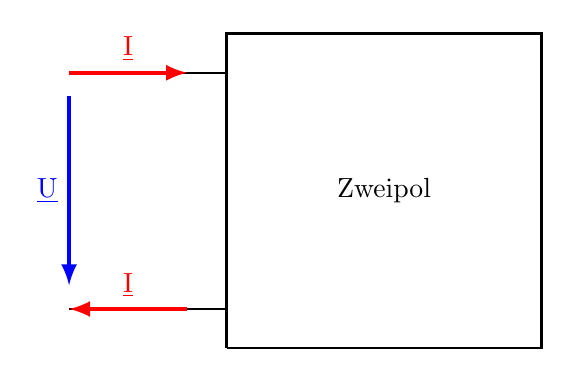
\begin{tikzpicture}
        \draw[thick] (-2, -2) |- (2, 2) |- (-2, -2);
        \node at (0, 0) {Zweipol};
        \draw[thick] (-4,  1.5) -- (-2,  1.5);
        \draw[thick] (-4, -1.5) -- (-2, -1.5);
        \draw[ultra thick, blue, -latex] (-4,  1.2) -- node[left]  {\underline{U}} (-4  , -1.2);
        \draw[ultra thick,  red, -latex] (-4,  1.5) -- node[above] {\underline{I}} (-2.5,  1.5);
        \draw[ultra thick,  red, latex-] (-4, -1.5) -- node[above] {\underline{I}} (-2.5, -1.5);
    \end{tikzpicture}
\end{figure}
Referenzpfeile für \underline{U} und \underline{I} gehen vom gleichen Pol aus. 
\[ \underline{S} = \underline{U} \cdot \underline{I}^\star = U \angle \varphi u \cdot I \angle -\varphi i \] 
\[ \underline{S} = \underbrace{U \cdot I}_{S} \angle \varphi_u - \varphi_i = P + j \cdot Q \]
\[ \varphi_u - \varphi_i = \varphi_z = \varphi_s \]
$\varphi_z$: Phasenlage einer Impedanz $Z \angle_z$

\begin{figure}[h!]
    \begin{tikzpicture}
        \draw[-latex] (-5, 0) -- (5, 0) node[right] {P};
        \draw[-latex] (0, -5) -- (0, 5) node[above] {Q};
        \draw[-latex, red] (0, 0) -- (20:4) node[above right] {\underline{S}};
        \draw[-latex] (1,0) node[above right, black] {$\varphi_s$} arc [radius = 1, start angle = 0, end angle = 20];
        \node[right] at (-4,  3) {Bezug von Q};
        \node[right] at (-4,  2) {Abgabe von P};
        \node[right] at (-4,  1) {$\to$ induktiv};
        \node[right] at ( 1,  3) {Bezug von Q};
        \node[right] at ( 1,  2) {Bezug von P};
        \node[right] at ( 1,  1) {$\to$ induktiv};
        \node[right] at (-4, -1) {Abgabe von Q};
        \node[right] at (-4, -2) {Abgabe von P};
        \node[right] at (-4, -3) {$\to$ kapazitiv};
        \node[right] at ( 1, -1) {Abgabe von Q};
        \node[right] at ( 1, -2) {Bezug von P};
        \node[right] at ( 1, -3) {$\to$ kapazitiv};
    \end{tikzpicture}
\end{figure}
\clearpage

\section{Erzeugerpfeilsystem}
\begin{figure}[h!]
    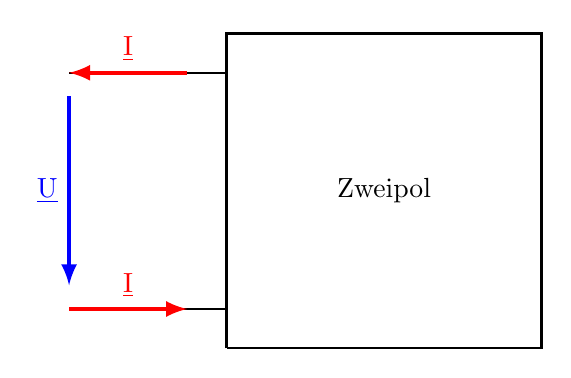
\begin{tikzpicture}
        \draw[thick] (-2, -2) |- (2, 2) |- (-2, -2);
        \node at (0, 0) {Zweipol};
        \draw[thick] (-4,  1.5) -- (-2,  1.5);
        \draw[thick] (-4, -1.5) -- (-2, -1.5);
        \draw[ultra thick, blue, -latex] (-4,  1.2) -- node[left]  {\underline{U}} (-4  , -1.2);
        \draw[ultra thick,  red, latex-] (-4,  1.5) -- node[above] {\underline{I}} (-2.5,  1.5);
        \draw[ultra thick,  red, -latex] (-4, -1.5) -- node[above] {\underline{I}} (-2.5, -1.5);
    \end{tikzpicture}
\end{figure}
Referenzpfeile für \underline{U} und \underline{I} gehen nicht vom gleichen Pol aus. 
\[ \underline{S} = \underline{U} \cdot \underline{I}^\star = U \angle \varphi u \cdot I \angle -\varphi i \] 
\[ \underline{S} = \underbrace{U \cdot I}_{S} \angle \varphi_u - \varphi_i = P + j \cdot Q \]

\begin{figure}[h!]
    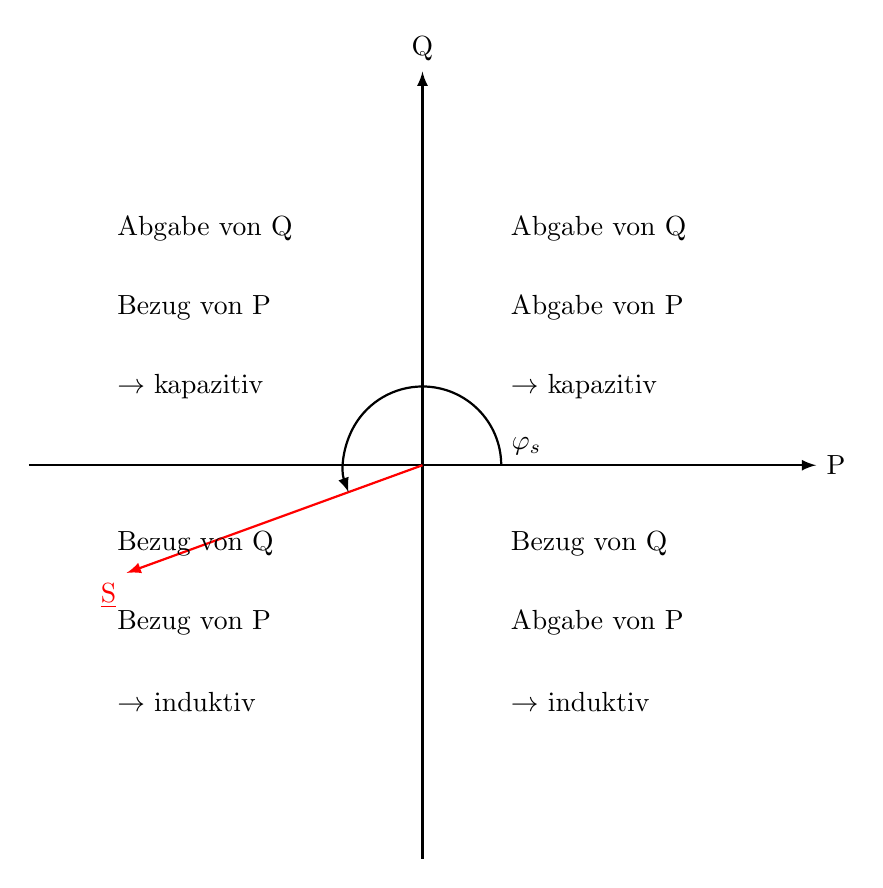
\begin{tikzpicture}
        \draw[-latex, thick] (-5, 0) -- (5, 0) node[right] {P};
        \draw[-latex, thick] (0, -5) -- (0, 5) node[above] {Q};
        \draw[-latex, thick, red] (0, 0) -- (200:4) node[below left] {\underline{S}};
        \draw[-latex, thick] (1,0) node[above right, black] {$\varphi_s$} arc [radius = 1, start angle = 0, end angle = 200];
        \node[right] at (-4,  3) {Abgabe von Q};
        \node[right] at (-4,  2) {Bezug von P};
        \node[right] at (-4,  1) {$\to$ kapazitiv};
        \node[right] at ( 1,  3) {Abgabe von Q};
        \node[right] at ( 1,  2) {Abgabe von P};
        \node[right] at ( 1,  1) {$\to$ kapazitiv};
        \node[right] at (-4, -1) {Bezug von Q};
        \node[right] at (-4, -2) {Bezug von P};
        \node[right] at (-4, -3) {$\to$ induktiv};
        \node[right] at ( 1, -1) {Bezug von Q};
        \node[right] at ( 1, -2) {Abgabe von P};
        \node[right] at ( 1, -3) {$\to$ induktiv};
    \end{tikzpicture}
\end{figure}
\clearpage

\subsection{Betriebsdiagramm des Generators}
EPS
\begin{figure}[h!]
    \begin{tikzpicture}
        \draw[-latex, thick] (-5, 0) -- (5, 0) node[right] {Q};
        \draw[-latex, thick] (0, -1) -- (0, 5) node[above] {P};
        \draw[thick] (4,0) arc [radius = 4, start angle = 0, end angle = 180];
    \end{tikzpicture}
\end{figure}

\end{document}
